
%\documentstyle[epsf,twocolumn]{jarticle}       %LaTeX2e仕様
% \documentclass[twocolumn]{jarticle}     %pLaTeX2e仕様(platex.exeの場合)
\documentclass[onecolumn]{ujarticle}   %pLaTeX2e仕様(uplatex.exeの場合)
%%%%%%%%%%%%%%%%%%%%%%%%%%%%%%%%%%%%%%%%%%%%%%%%%%%%%%%%%%%%%%
%%
%%  基本バージョン
%%
%%%%%%%%%%%%%%%%%%%%%%%%%%%%%%%%%%%%%%%%%%%%%%%%%%%%%%%%%%%%%%%%
\setlength{\topmargin}{-45pt}
%\setlength{\oddsidemargin}{0cm}
\setlength{\oddsidemargin}{-7.5mm}
%\setlength{\evensidemargin}{0cm}
\setlength{\textheight}{24.1cm}
%setlength{\textheight}{25cm}
\setlength{\textwidth}{17.4cm}
%\setlength{\textwidth}{172mm}
\setlength{\columnsep}{11mm}

%\kanjiskip=.07zw plus.5pt minus.5pt


% 【節が変わるごとに (1.1)(1.2) … (2.1)(2.2) と数式番号をつけるとき】
%\makeatletter
%\renewcommand{\theequation}{%
%\thesection.\arabic{equation}} %\@addtoreset{equation}{section}
%\makeatother

%\renewcommand{\arraystretch}{0.95} 行間の設定
%%%%%%%%%%%%%%%%%%%%%%%%%%%%%%%%%%%%%%%%%%%%%%%%%%%%%%%%
%\usepackage{graphicx}   %pLaTeX2e仕様(\documentstyle ->\documentclass)
\usepackage[dvipdfmx]{graphicx}
\usepackage{subcaption}
\usepackage{multirow}
\usepackage{amsmath}
\usepackage{url}
\usepackage{ulem}
\usepackage{algorithm}
\usepackage{algorithmic}
\usepackage{listings} %,jlisting} %日本語のコメントアウトをする場合jlistingが必要
%ここからソースコードの表示に関する設定
\lstset{
  basicstyle={\ttfamily},
  identifierstyle={\small},
  commentstyle={\smallitshape},
  keywordstyle={\small\bfseries},
  ndkeywordstyle={\small},
  stringstyle={\small\ttfamily},
  frame={tb},
  breaklines=true,
  columns=[l]{fullflexible},
  numbers=left,
  xrightmargin=0zw,
  xleftmargin=3zw,
  numberstyle={\scriptsize},
  stepnumber=1,
  numbersep=1zw,
  lineskip=-0.5ex
}
\newcommand{\argmax}{\mathop{\rm arg~max}\limits}
\newcommand{\argmin}{\mathop{\rm arg~min}\limits}

%%%%%%%%%%%%%%%%%%%%%%%%%%%%%%%%%%%%%%%%%%%%%%%%%%%%%%%%
\begin{document}

	%bibtex用の設定
	%\bibliographystyle{ujarticle}

	% \twocolumn[
		\noindent
		\hspace{1em}
		2022 年 6 月 17 日
		ゼミ資料
		\hfill
		杉山 竜弥
		\vspace{2mm}

		\hrule
		\begin{center}
			{\Large \bf 進捗報告}
		\end{center}
		\hrule
		\vspace{9mm}
	% ]


\section{今週やったこと}
\begin{itemize}
  \item Sketchformer
  \item スケッチ分割
  \item AKAZE
\end{itemize}


\section{Sketchformerの準備}
マルチクラスに対応して,事前学習パラメータも用意されている.
データセットを専用の形式に変換するのに時間がかかっているが,
終わり次第今までの実験を Sketchformer でやりたい.


\section{スケッチ分割実験}

オリジナルスケッチをスケッチ1, スケッチ2に分割し,デコードした $z_1 + z_2$ と比較した.
結果としてオリジナルと離れたスケッチが出力された.
エンコードがうまくできていないため,潜在変数を足した場合が崩れたと考えられる.


\begin{figure}[th]
  \begin{center}
    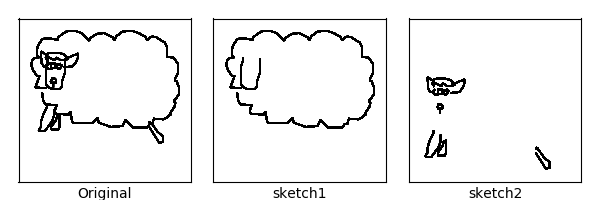
\includegraphics[clip,width=100mm]{sketch_trained_split_6.png}
    \caption{オリジナル/分割後1/分割後2}
    \label{fig:result1_1}
  \end{center}
\end{figure}

\begin{figure}[th]
  \begin{center}
    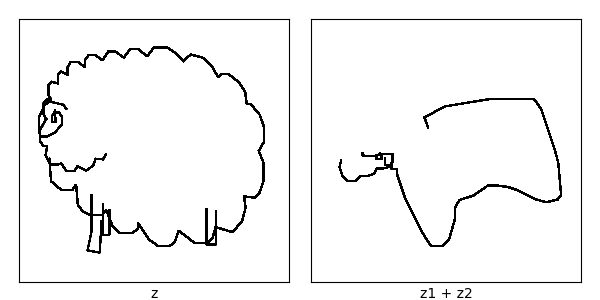
\includegraphics[clip,width=60mm]{sketch_trained_split_6_rec.png}
    \caption{オリジナルデコード/分割後1+2デコード}
    \label{fig:result1_2}
  \end{center}
\end{figure}


\section{AKAZE での類似度比較}
ラスタ画像化したスケッチを AKAZE で類似度比較した.
あるスケッチからデコードしたものを比較元として,
オリジナルを含む 10 枚のスケッチと AKAZE 類似度を出した.
図 \ref{fig:result2_1} ~ \ref{fig:result2_4} に示す.
主観ではスケッチでも十分類似度として機能していると感じた.
最終状態の類似度比較指標は AKAZE の利用を検討している.


\begin{figure}[htbp]
    \begin{tabular}{cc}
      \begin{minipage}[t]{0.45\hsize}
        \centering
        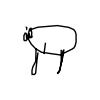
\includegraphics[keepaspectratio, scale=0.8]{decode1.png}
        \caption{比較元のデコードスケッチ}
        \label{fig:result2_1}
      \end{minipage} &
      \begin{minipage}[t]{0.45\hsize}
        \centering
        
\includegraphics[keepaspectratio, scale=0.8]{encode1.png}
        \caption{オリジナルスケッチ D=111}
        \label{fig:result2_2}
      \end{minipage} \\

      \begin{minipage}[t]{0.45\hsize}
        \centering
        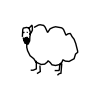
\includegraphics[keepaspectratio, scale=0.8]{encode8.png}
        \caption{最小AKAZE類似度スケッチ D=95}
        \label{fig:result2_3}
      \end{minipage} &
      \begin{minipage}[t]{0.45\hsize}
        \centering
        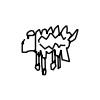
\includegraphics[keepaspectratio, scale=0.8]{encode9.png}
        \caption{最大AKAZE類似度スケッチ D=124}
        \label{fig:result2_4}
      \end{minipage}
    \end{tabular}
  \end{figure}


\section{予定}
描き順と最終状態の類似度指標を一旦完成させ,
さらに絵描き歌用のオブジェクトへ分割するところまでいきたい.

その次の週は資料作成と発表準備.

% \begin{figure}[h]
%   \begin{center}
%     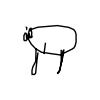
\includegraphics[clip,width=20mm]{decode1.png}
%     \caption{比較元のデコードスケッチ}
%     \label{fig:result2_1}
%   \end{center}
% \end{figure}

% 参考文献リスト
% \bibliographystyle{unsrt}
% \bibliography{ref}
\end{document}
